\chapter{Approach}\label{chap:chap4}

\section*{}
This chapter focus on the description of the approach used to solve the
problem presented for this thesis. It begins with an high level architecture
description and a brief description of the main phases that take part of the
proposed approach.

This section is followed by a more low level architecture of each one of the phases.
Of each phase, its main flow is described, its principal variables, constrains and
used methods, algorithms and their objective.

It concludes with a description of the experimental setup for the whole approach
and for each component; this last part is an introduction to the next
chapter where the results are discussed and analysed.

\section{High-level Architecture}

\begin{figure}[h] \begin{center} \leavevmode
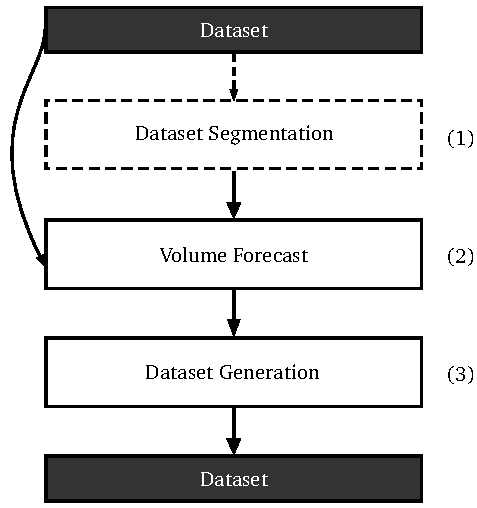
\includegraphics[]{high_level} \caption{ High level overview
of the approach } \label{fig:highlevel_arch} \end{center} \end{figure}

As the figure~\ref{fig:highlevel_arch} makes clear, the goal of the
proposed approach is to use a past dataset containing the log of the web
activity of an online advertising related network to generate a representation of a
possible future web activity on the same network. In such a way, that the
tendencies and the data coherency is preserved.

This approach can be divided three main phases, the first, \emph{segmentation}, is
optional, its main purpose is divide the dataset in smaller and more predictable
datasets in order to improve the results of the second phase, mostly when there
are large quantities of data available.

The second phase is where the \emph{forecast of the volumes} that characterize the traffic on
the network are done, using time series prediction method.

The third an last phase of the process, the more complex one, is where the volumes
generated from the phase two combined with the data provided by the original
dataset are used to \emph{generate a dataset} that represent a possible future of the
web activity on the target network.

\section{Architecture for Web Activity Forecasting and Synthesising}

\subsection{Data Segmentation}

\begin{figure}[h] \begin{center} \leavevmode
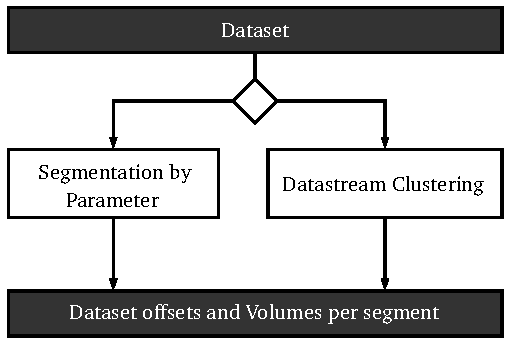
\includegraphics[]{segmentation} \caption{ High level overview
of Data Segmentation} \label{fig:segmentation_arch} \end{center} \end{figure}

Goals:
- Try to give more granularity to the time series 
- Try to aggregate similar data in order to make it more predictable

How its done:
- parameters:
 - able to be use datasets from different sources no param is garanted to be
 available so it is configurable. 
   -Pros:
     -Can achive great results if enough data and seasonal data available 
  - Cons:
    - Manual selection of the parameters
- Datastream
  - based on join similar entries together.
  - Main disadvantage no garantee that similar data gives better results

\subsection{Volume Forecasting}

-Explain the metrics selected:
 - number impressions
 - percentage of uniques vs number  uniques
 - percentage of new entries
Usage of arima

\subsection{Dataset Generator}

\begin{figure}[h] \begin{center} \leavevmode
\includegraphics[]{high_level_file_gen} \caption{ High level overview
of the Dataset Generator } \label{fig:highlevel_arch_file_gen} \end{center} \end{figure}

palceholder

\subsubsection{Pre-process (i)}

\begin{figure}[h] \begin{center} \leavevmode
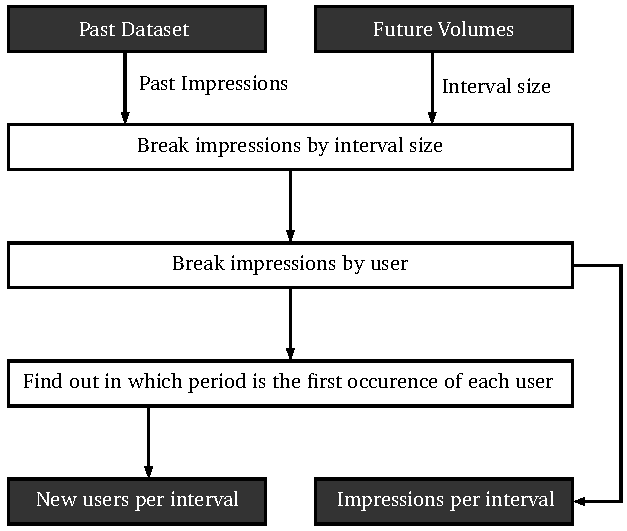
\includegraphics[]{pre_processing_i} \caption{ High level overview
of the Dataset Pre-processing} \label{fig:pre_processing_i} \end{center} \end{figure}

palceholder

\subsubsection{Calculate Statistics (ii)}

\begin{figure}[h] \begin{center} \leavevmode
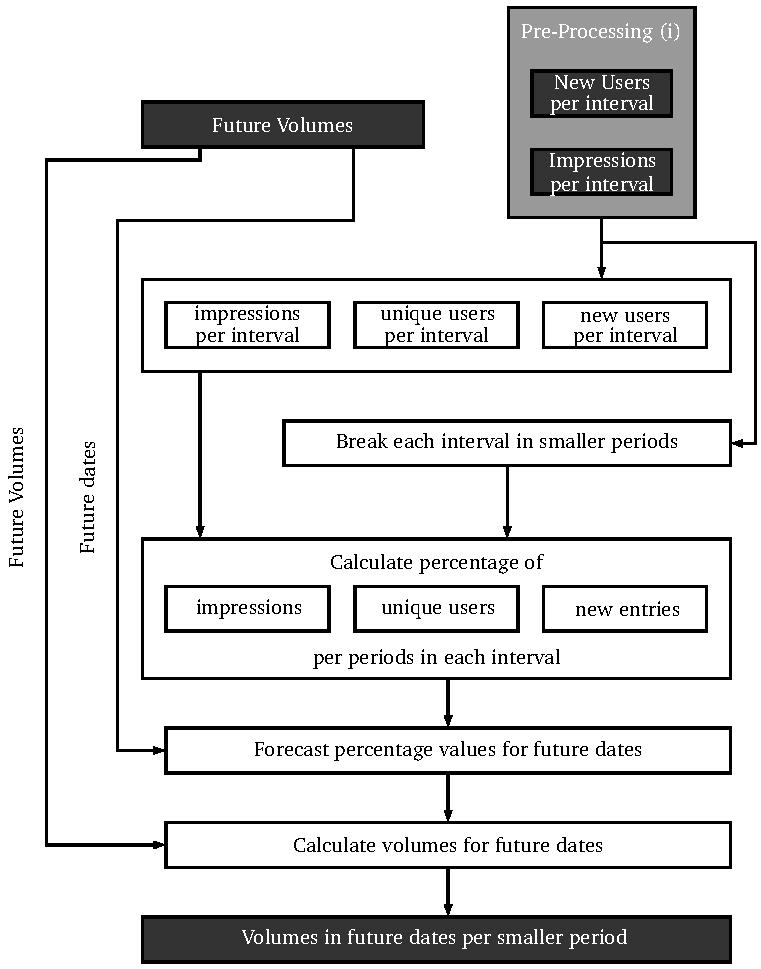
\includegraphics[]{calculate_stats} \caption{ High level overview
of statistics calculation} \label{fig:calculate_stats_ii} \end{center} \end{figure}

palceholder

\subsubsection{Fill Future Data (iii)}

\begin{figure}[h] \begin{center} \leavevmode
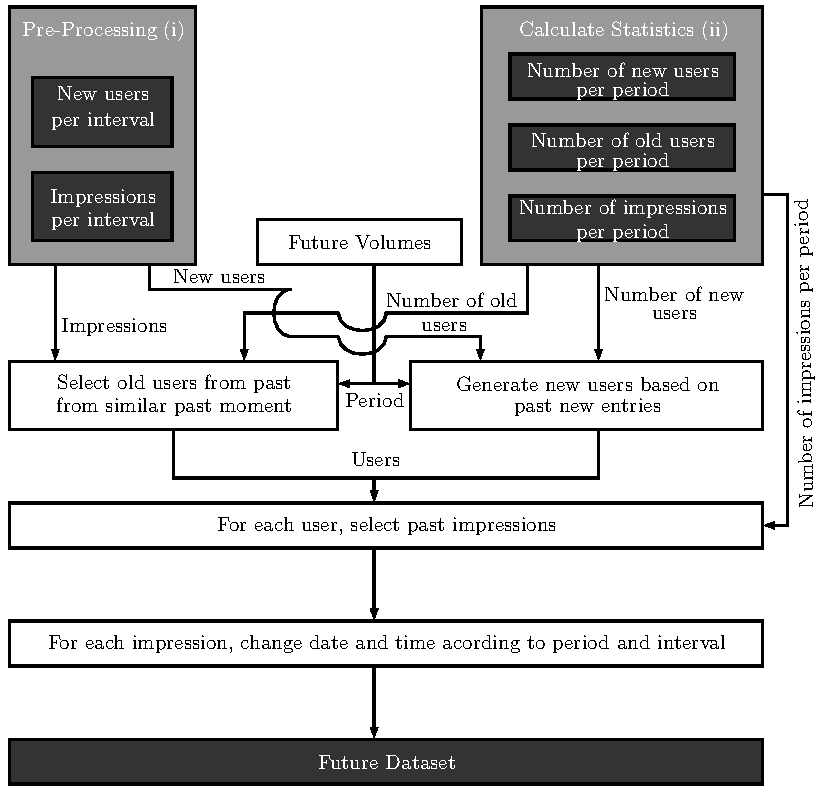
\includegraphics[]{fill_future} \caption{ High level overview
of fill future data} \label{fig:fill_future_iii} \end{center} \end{figure}

placeholder


\section{Component Testing}

\subsection{Data Segmentation}

\subsection{Volume Forecasting}

\subsection{Dataset Generator}


\section{Results and Conclusions}

